\subsection{Kreuzkorrelationsfunktion}
\textit{verfasst von Lucas Weber\\}
Die Basis f"ur die Bemessung der aufgenommenen Audiosignale bildet die sogenannte Kreuzkorrelationsfunktion (KKF). Wie in der Aufgabenstellung schon beschrieben werden an ihr die Bemessungsparameter festgelegt. Aufgrund der verschiedenen Blockl"angen und der Masse an Daten, die korreliert werden sollen muss die Berechnung der KKF effizient und zeitsparend implementiert werden. Im Folgenden Abschnitt wird die KKF kurz theoretisch eingef"uhrt und das das mathematische Konzept erkl"art, auf dem die effiziente Berechnung der KKF beruht.
\\\\
Zuerst haben wir f"ur die KKF eine Funktion genutzt, die zur Berechnung Summen verwendete. Dabei ergab sich, dass die Berechnung zu langsam war. In der nun vorliegenden Octave-Version wird die KKF im Frequenzbereich berechnet.
\subsubsection{Berechnungsvorschrift}
Die KKF ist als aus zwei verschiedenen Funktionen gebildeter Erwartungswert definiert. Hier werden die Formeln allgemein f"ur die Korrelation der Prozesse \textbf{X} und \textbf{Y} angegeben.[ISV, S. 84] 

\begin{align}
\psi_{\textbf XY}(t_1, t_2) = E\lbrace\textbf{X}(t_1)\cdot\textbf{Y}(t_2)\rbrace\\\text{[ISV, S. 84 Formel 2.200]}
\end{align}
Dadurch dass sich der Raum, das Wiedergabemedium und die Aufnahmeart während der Aufnahme nicht geändert haben, können die Prozesse als schwach stationär angenommen werden. Außerdem wird angenommen, dass die Prozesse ergodisch sind. Durch diese Voraussetzungen hängt die KKF nicht mehr von einer Verschiebung zu bestimmten Zeitpunkten $(t_1 - t_2)$ ab sondern nur noch von ihrer Verschiebung $\tau$ . Reale, aufgenommene Audiosignale s(t), die hier mit durch die KKF verrechnet werden, sind in jedem Fall Energiesignale, da sie rein reell sind, einen begrenzten Wertebereich haben und nach einer bestimmten Zeit enden.[vgl. ISV, S. 85 f]

\begin{align}
Signalenergie := \int_{-\infty}^{\infty} s^2(t) \,dt < \infty
\end{align}

\noindent Da die aufgenommenen Audiosignale zeit-diskrete Energiesignale sind wird hier auch nur die zeit-diskrete Kreuzkorrelation beschrieben. F"ur zeit-diskrete Energiesignale ergibt sich die folgende Berechnungsvorschrift, wobei x(n) und y(n) diskrete Realisierungen der Prozesse \textbf{X} und \textbf{Y} sind.[ISV, S. 88 f]

\begin{align}
\boxed{\psi_{\textbf {XY}}^E(k) = \sum_{n = -\infty}^{\infty} x(n) \cdot y(n+k)}\\\text{[ISV, S. 89 Formel 2.218]}
\end{align}

\subsubsection{Kreuzkorrelation im Frequenzbereich und Faltungssatz}
Am Anfang unserer Arbeit haben wir uns mit der Berechnung der Kreuzkorrelation besch"aftigt. Da die Bildung der Summe der Multiplikation von x(n) und y(n+k) sehr rechenaufw"andig ist, haben wir nach schnelleren M"oglichkeiten gesucht die KKF der beiden Signale zu berechnen. Eine geeignet M"oglichkeit ist die Berechnung der KKF im Frequenzbereich. F"ur die Berechnung der KKF im Frequenzbereich macht man sich die "Ahnlichkeit der KKF zur Faltung und den Faltungssatz zunutze.

\paragraph{KKF als Faltung}\textbf{\\\\Zeit-kontinuierlicher Fall:}
\begin{align}
\psi_{\textbf {XY}}^E(\tau) = x(-\tau) * y(\tau)\\\text{[ISV, S. 89 Formel 2.217]}
\end{align}
\textbf{Zeit-diskreter Fall:}
\begin{align}
\psi_{\textbf {XY}}^E(k) = x(-k) * y(k)
\end{align}
\paragraph{Faltungssatz in Verbindung mit KKF}Wir schreiben zuerst die die KKF als Faltung. Danach transformieren wir die Faltung in den Frequenzbereich. Durch geschicktes Erweitern und Substitution findet man einen Ausdruck, um die KKF im Frequenzbereich zu berechnen.

\begin{align}
\psi(t) \  \; &= x(-t) * y(t) = \int_{-\infty}^{\infty} x(-\tau) \cdot y(t-\tau)\,d\tau\\\\
\underline \Psi(\omega) &=\int_{-\infty}^{\infty} x(-t) * y(t) \cdot e^{-j\omega t} \,dt\\&=\int_{-\infty}^{\infty} \left[ \int_{-\infty}^{\infty} x(-\tau) \cdot y(t-\tau)\,d\tau \right] \cdot e^{-j\omega (t - \tau + \tau)} \,dt\\&=\int_{-\infty}^{\infty} x(-\tau) \cdot e^{-j\omega(\tau)} \underbrace{ \left[ \int_{-\infty}^{\infty} y(t-\tau) e^{-j\omega (t - \tau)} \,dt \right]}_* \,d\tau
\end{align}
Durch Substitution von $(t-\tau)$ durch $t'$ ergibt sich * zur Fourier-transformierten $ \underline{Y}(\omega)$ von y(t). Der restliche Ausdruck wird wegen der folgenden Beziehung zur Transformierten $ \underline{X}^*(\omega)$ der Funktion x(t).
\begin{align}
s^*(-t) = S^*(f)\text{[NT, S. 103 Korrespondenztabelle]}
\end{align}
$s(t)$ ist unserem Fall rein reell ist, wodurch sich der Ausdruck deswegen zu
\begin{align}
s^*(-t) = s(-t) = S^*(f)
\end{align}
vereinfacht.

\\\\
Die KKF l"asst sich im Frequenzbereich also als

\begin{align}
\boxed{\underline \Psi(\omega) = \underline{X}^*(\omega) \cdot \underline{Y}(\omega)}
\end{align}
schreiben. [ISV, S.180]
\\\\
Wenn man nun die KKF im Frequenzbereich zeitsparend durchf"uhren will, muss man die FFT f"ur x(k) und y(k) (dabei $k \in \mathbb{N}^+_0$) der L"ange N durchf"uhren. Dabei muss man beachten, dass bei der FFT ein Linienspektrum ergibt. Die FFT beruht vor allem auch auf der Annahme, dass sich die N diskreten Werte periodisch wiederholen [ISV, S.135]. Durch die IFFT von $ \underline \Psi(\omega)$ ergibt sich also die periodische KKF $\tilde{\psi}(t)$.
\subsubsection{Zero Padding}
Die periodische KKF $\tilde{\psi}(t)$ ist in unserem Projekt zudem die bessere Wahl. Berechnet man die KKF im Frequenzbereich wird durch die implementierten Funktionen von Octave, so wie von Python, sogenanntes Zero-Padding durchgeführt. Vorstellen kann man sich das als auffüllen der Daten mit N Werten $=0$ an jeweils den Rändern einer der beiden Funktionen, da durch die Verschiebung eine der Funktionen über den Rand der anderen hinausragt.
\begin{figure}[ht!] 
  \centering
     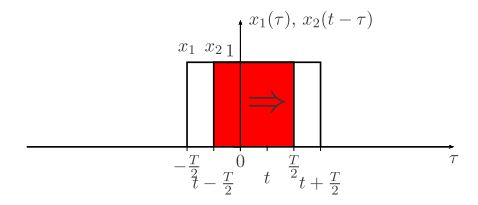
\includegraphics[width=0.4\textwidth]{img/Faltung}
  \caption{Anschauliches Beispiel zur Faltung [NT, S. 28]}
  \label{fig:Bild1}
\end{figure}
Wie man in Abbildung \ref{fig:Bild1} erkennen kann ist die Funktion $x_2$ soweit verschoben, dass sie über den rechten Rand der Funktion $x_1$ hinausragt. Wenn man die beiden Rechtecksignale als Bereiche sieht in denen echte Funktionswerte liegen, würde nun auf der positiven x-Achse ab $T/2$ mit Nullen aufgefüllt werden. Dadurch bekommt die KKF automatisch ein Abklingverhalten an ihren Rändern, das nur durch die begrenzte Anzahl an Werten verursacht wird. Die Korrelation nimmt an den Rändern nicht zwingend ab. Durch dieses Abklingverhalten würden unsere Ergebnisse also abgefälscht werden. Die periodische KKF ist also aussagekräftiger, da unser reales Signal in jedem Fall an den Rändern der korrelierten Blöcke nicht auf Null abklingt.Wenn man die periodische KKF im Zeitbereich berechnen möchte, müsste man an den Rändern der Funktionen nochmal die Funktion $x_1$ anhängen.
